% Important: If latex complains about unicode characters, please use "\usepackage[utf8x]{inputenc}" in your preamble
% You can change the size of the picture by putting it into the construct:
% 1) \resizebox{10cm}{!}{"below picture"} to scale horizontally to 10 cm
% 2) \resizebox{!}{15cm}{"below picture"} to scale vertically to 15 cm
% 3) \resizebox{10cm}{15cm}{"below picture"} a combination of above two
% It is not recomended to use the scale option of the tikzpicture environment.
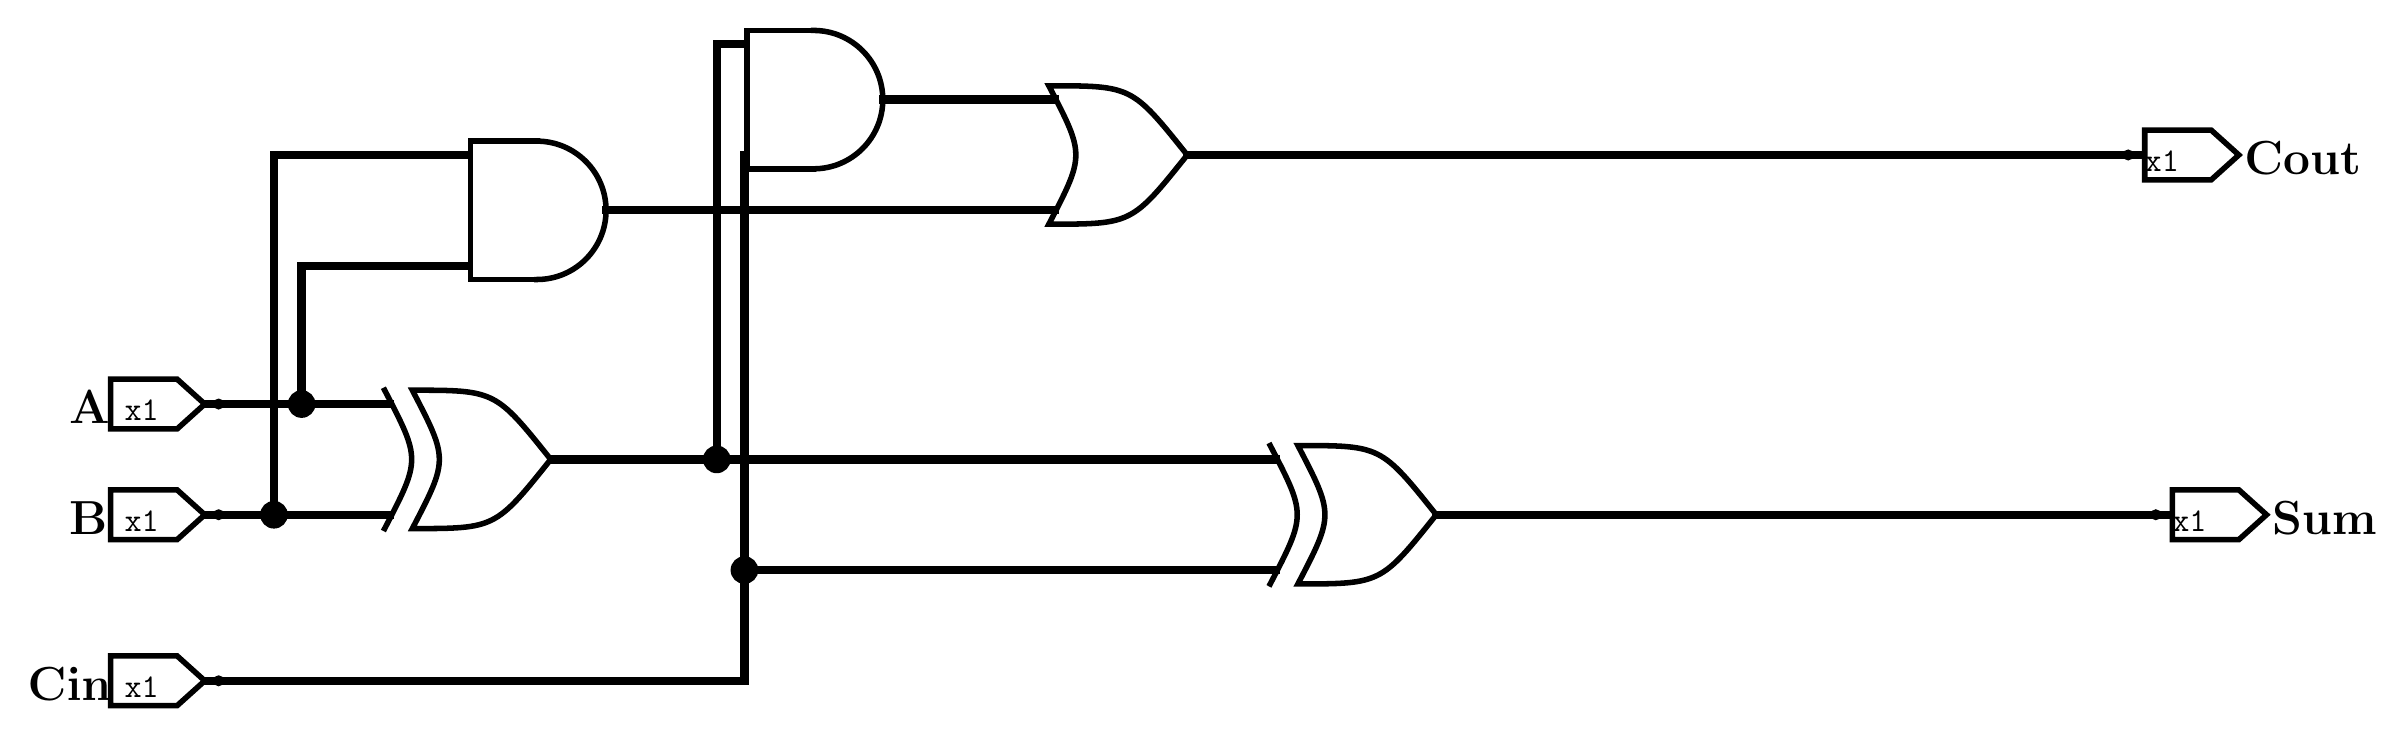
\begin{tikzpicture}[x=1pt,y=-1pt,line cap=rect]
\def\logisimfontA#1{\fontfamily{cmr}{#1}} % Replaced by logisim, original font was "SansSerif"
\def\logisimfontB#1{\fontfamily{cmtt}{#1}} % Replaced by logisim, original font was "Monospaced"
\definecolor{custcol_0_0_0}{RGB}{0, 0, 0}
\definecolor{custcol_ff_ff_ff}{RGB}{255, 255, 255}
\draw [line width=3.0pt, custcol_0_0_0 ]  (424.0,50.0) -- (764.0,50.0) ;
\draw [line width=3.0pt, custcol_0_0_0 ]  (164.0,90.0) -- (104.0,90.0) -- (104.0,140.0) ;
\draw [line width=3.0pt, custcol_0_0_0 ]  (264.0,50.0) -- (264.0,200.0) ;
\draw [line width=3.0pt, custcol_0_0_0 ]  (194.0,160.0) -- (254.0,160.0) -- (254.0,10.0) -- (264.0,10.0) ;
\draw [line width=3.0pt, custcol_0_0_0 ]  (514.0,180.0) -- (774.0,180.0) ;
\fill [line width=3.0pt, custcol_0_0_0]  (94.0,180.0) ellipse (5.0 and 5.0 );
\fill [line width=3.0pt, custcol_0_0_0]  (254.0,160.0) ellipse (5.0 and 5.0 );
\fill [line width=3.0pt, custcol_0_0_0]  (104.0,140.0) ellipse (5.0 and 5.0 );
\fill [line width=3.0pt, custcol_0_0_0]  (264.0,200.0) ellipse (5.0 and 5.0 );
\draw [line width=3.0pt, custcol_0_0_0 ]  (314.0,30.0) -- (374.0,30.0) -- (376.0,30.0) ;
\draw [line width=3.0pt, custcol_0_0_0 ]  (214.0,70.0) -- (374.0,70.0) -- (376.0,70.0) ;
\draw [line width=2.0pt, custcol_0_0_0 ]  (424.0,50.0) .. controls  (404.0,25.0)  ..  (374.0,25.0) .. controls  (387.0,50.0)  ..  (374.0,75.0) .. controls  (404.0,75.0)  ..  (424.0,50.0) -- cycle ;
\draw [line width=3.0pt, custcol_0_0_0 ]  (254.0,160.0) -- (454.0,160.0) -- (456.0,160.0) ;
\draw [line width=2.0pt, custcol_0_0_0 ]  (514.0,180.0) .. controls  (494.0,155.0)  ..  (464.0,155.0) .. controls  (477.0,180.0)  ..  (464.0,205.0) .. controls  (494.0,205.0)  ..  (514.0,180.0) -- cycle ;
\draw [line width=2.0pt, custcol_0_0_0 ]  (454.0,155.0) .. controls  (467.0,180.0)  ..  (454.0,205.0) ;
\draw [line width=2.0pt, custcol_0_0_0] (289.0,55.0) arc (90.0:-90.0:25.0 and 25.0 );
\draw [line width=2.0pt, custcol_0_0_0 ]  (289.0,5.0) -- (265.0,5.0) -- (265.0,55.0) -- (289.0,55.0) ;
\draw [line width=2.0pt, custcol_0_0_0] (189.0,95.0) arc (90.0:-90.0:25.0 and 25.0 );
\draw [line width=2.0pt, custcol_0_0_0 ]  (189.0,45.0) -- (165.0,45.0) -- (165.0,95.0) -- (189.0,95.0) ;
\draw [line width=3.0pt, custcol_0_0_0 ]  (94.0,180.0) -- (134.0,180.0) -- (136.0,180.0) ;
\draw [line width=2.0pt, custcol_0_0_0 ]  (194.0,160.0) .. controls  (174.0,135.0)  ..  (144.0,135.0) .. controls  (157.0,160.0)  ..  (144.0,185.0) .. controls  (174.0,185.0)  ..  (194.0,160.0) -- cycle ;
\draw [line width=2.0pt, custcol_0_0_0 ]  (134.0,135.0) .. controls  (147.0,160.0)  ..  (134.0,185.0) ;
\draw [line width=3.0pt, custcol_0_0_0 ]  (778.0,180.0) -- (775.0,180.0) ;
\draw [line width=2.0pt, custcol_0_0_0 ]  (804.0,171.0) -- (814.0,180.0) -- (804.0,189.0) -- (780.0,189.0) -- (780.0,171.0) -- cycle;
\logisimfontB{\fontsize{12pt}{12pt}\selectfont\node[inner sep=0, outer sep=0, custcol_0_0_0, anchor=base west] at  (780.0,186.0)  {x1};}
\logisimfontA{\fontsize{16pt}{16pt}\fontseries{bx}\selectfont\node[inner sep=0, outer sep=0, custcol_0_0_0, anchor=base west] at  (816.0,187.0)  {Sum};}
\fill [line width=2.0pt, custcol_0_0_0]  (774.0,180.0) ellipse (2.0 and 2.0 );
\draw [line width=3.0pt, custcol_0_0_0 ]  (69.0,140.0) -- (74.0,140.0) -- (104.0,140.0) -- (134.0,140.0) -- (136.0,140.0) ;
\draw [line width=2.0pt, custcol_0_0_0 ]  (59.0,149.0) -- (69.0,140.0) -- (59.0,131.0) -- (35.0,131.0) -- (35.0,149.0) -- cycle;
\logisimfontB{\fontsize{12pt}{12pt}\selectfont\node[inner sep=0, outer sep=0, custcol_0_0_0, anchor=base west] at  (40.0,146.0)  {x1};}
\logisimfontA{\fontsize{16pt}{16pt}\fontseries{bx}\selectfont\node[inner sep=0, outer sep=0, custcol_0_0_0, anchor=base west] at  (20.0,147.0)  {A};}
\fill [line width=2.0pt, custcol_0_0_0]  (74.0,140.0) ellipse (2.0 and 2.0 );
\draw [line width=3.0pt, custcol_0_0_0 ]  (69.0,180.0) -- (74.0,180.0) -- (94.0,180.0) -- (94.0,50.0) -- (164.0,50.0) ;
\draw [line width=2.0pt, custcol_0_0_0 ]  (59.0,189.0) -- (69.0,180.0) -- (59.0,171.0) -- (35.0,171.0) -- (35.0,189.0) -- cycle;
\logisimfontB{\fontsize{12pt}{12pt}\selectfont\node[inner sep=0, outer sep=0, custcol_0_0_0, anchor=base west] at  (40.0,186.0)  {x1};}
\logisimfontA{\fontsize{16pt}{16pt}\fontseries{bx}\selectfont\node[inner sep=0, outer sep=0, custcol_0_0_0, anchor=base west] at  (20.0,187.0)  {B};}
\fill [line width=2.0pt, custcol_0_0_0]  (74.0,180.0) ellipse (2.0 and 2.0 );
\draw [line width=3.0pt, custcol_0_0_0 ]  (768.0,50.0) -- (765.0,50.0) ;
\draw [line width=2.0pt, custcol_0_0_0 ]  (794.0,41.0) -- (804.0,50.0) -- (794.0,59.0) -- (770.0,59.0) -- (770.0,41.0) -- cycle;
\logisimfontB{\fontsize{12pt}{12pt}\selectfont\node[inner sep=0, outer sep=0, custcol_0_0_0, anchor=base west] at  (770.0,56.0)  {x1};}
\logisimfontA{\fontsize{16pt}{16pt}\fontseries{bx}\selectfont\node[inner sep=0, outer sep=0, custcol_0_0_0, anchor=base west] at  (806.0,57.0)  {Cout};}
\fill [line width=2.0pt, custcol_0_0_0]  (764.0,50.0) ellipse (2.0 and 2.0 );
\draw [line width=3.0pt, custcol_0_0_0 ]  (69.0,240.0) -- (74.0,240.0) -- (264.0,240.0) -- (264.0,200.0) -- (454.0,200.0) -- (456.0,200.0) ;
\draw [line width=2.0pt, custcol_0_0_0 ]  (59.0,249.0) -- (69.0,240.0) -- (59.0,231.0) -- (35.0,231.0) -- (35.0,249.0) -- cycle;
\logisimfontB{\fontsize{12pt}{12pt}\selectfont\node[inner sep=0, outer sep=0, custcol_0_0_0, anchor=base west] at  (40.0,246.0)  {x1};}
\logisimfontA{\fontsize{16pt}{16pt}\fontseries{bx}\selectfont\node[inner sep=0, outer sep=0, custcol_0_0_0, anchor=base west] at  (5.0,247.0)  {Cin};}
\fill [line width=2.0pt, custcol_0_0_0]  (74.0,240.0) ellipse (2.0 and 2.0 );
\end{tikzpicture}

